% !TeX program = xelatex
% !TeX encoding = UTF-8
\documentclass[14pt,a4paper,oneside]{extreport}

% ================================================================
% Báo cáo Hệ thống nhận dạng biển số xe ô tô bằng trí tuệ nhân tạo
% Compiler: XeLaTeX, chạy ít nhất 2 lần để cập nhật mục lục.
% ================================================================

\usepackage{iftex}
\ifPDFTeX
  \usepackage[utf8]{vietnam}
  \usepackage{newtxtext,newtxmath}
\else
  \usepackage{fontspec}
  \defaultfontfeatures{Ligatures=TeX}
  \IfFontExistsTF{Times New Roman}{
    \setmainfont{Times New Roman}[
      BoldFont={Times New Roman Bold},
      ItalicFont={Times New Roman Italic},
      BoldItalicFont={Times New Roman Bold Italic}
    ]
  }{
    \setmainfont{TeX Gyre Termes}
  }
\fi

\usepackage{geometry}
\geometry{a4paper,top=2.5cm,bottom=2.5cm,left=3cm,right=2cm,headsep=0.65cm,footskip=1cm}

\usepackage{setspace}
\setstretch{1.2}
\setlength{\parindent}{1.27cm}
\setlength{\parskip}{3pt}
\setlength{\emergencystretch}{2em}
\usepackage{indentfirst}
\usepackage{microtype}

\usepackage{graphicx}
\usepackage{float}
\usepackage{pdflscape}
\usepackage{longtable}
\usepackage{array}
\usepackage{tabularx}
\usepackage{ragged2e}
\usepackage{multirow}
\usepackage{booktabs}
\usepackage{enumitem}
\usepackage{titlesec}
\usepackage{fancyhdr}
\usepackage{caption}
\usepackage{xcolor}
\usepackage{tikz}
\usetikzlibrary{arrows.meta,calc,fit,positioning,shapes.geometric,backgrounds}
\usepackage{hyperref}
\usepackage{etoolbox}
\usepackage{xparse}
\usepackage{listings}
\usepackage{amsmath}

% ================================================================
% Màu sắc
% ================================================================
\definecolor{reportblue}{RGB}{0,102,204}
\definecolor{lightgray}{gray}{0.94}
\definecolor{midgray}{gray}{0.55}
\definecolor{darkgray}{gray}{0.20}
\definecolor{codegray}{RGB}{248,248,248}
\definecolor{codegreen}{RGB}{0,128,0}
\definecolor{codepurple}{RGB}{128,0,128}
\definecolor{codeblue}{RGB}{0,0,200}

% ================================================================
% Bảng
% ================================================================
\setlength{\arrayrulewidth}{0.6pt}
\setlength{\tabcolsep}{5pt}
\renewcommand{\arraystretch}{1.25}

% ================================================================
% Hyperref
% ================================================================
\hypersetup{
  unicode=true,
  colorlinks=false,
  hidelinks,
  pdfborder={0 0 0},
  pdfauthor={Nhóm sinh viên},
  pdftitle={Hệ thống nhận dạng biển số xe ô tô bằng trí tuệ nhân tạo}
}
\urlstyle{same}

% ================================================================
% Định dạng tiêu đề
% ================================================================
\renewcommand{\chaptername}{CHƯƠNG}
\titleformat{\chapter}[block]
  {\centering\bfseries\fontsize{18pt}{22pt}\selectfont}
  {\chaptername~\thechapter.}
  {0.7em}
  {\MakeUppercase}
\titlespacing*{\chapter}{0pt}{20pt}{15pt}

\titleformat{\section}
  {\bfseries\fontsize{16pt}{19pt}\selectfont}
  {\thesection.}{0.7em}{}
\titleformat{\subsection}
  {\bfseries\fontsize{14pt}{17pt}\selectfont}
  {\thesubsection.}{0.7em}{}
\titleformat{\subsubsection}
  {\bfseries\itshape\fontsize{14pt}{17pt}\selectfont}
  {\thesubsubsection.}{0.7em}{}

\titlespacing*{\section}{0pt}{1.0em}{0.5em}
\titlespacing*{\subsection}{0pt}{0.8em}{0.4em}
\titlespacing*{\subsubsection}{0pt}{0.7em}{0.3em}

\renewcommand{\contentsname}{MỤC LỤC}
\renewcommand{\listtablename}{DANH MỤC BẢNG}
\renewcommand{\listfigurename}{DANH MỤC HÌNH}
\renewcommand{\tablename}{Bảng}
\renewcommand{\figurename}{Hình}
\renewcommand{\bibname}{TÀI LIỆU THAM KHẢO}
\setcounter{tocdepth}{3}
\setcounter{secnumdepth}{3}

\captionsetup{font=normalsize,labelfont=bf,justification=centering}
\captionsetup[table]{position=top,skip=6pt}
\captionsetup[figure]{position=bottom,skip=6pt}

\setlist[itemize]{leftmargin=1.1cm,label=--,itemsep=0.2em,topsep=0.3em}
\setlist[enumerate]{leftmargin=1.1cm,itemsep=0.2em,topsep=0.3em}

% ================================================================
% Style code listing -- Java + Bash
% ================================================================
\lstdefinestyle{javastyle}{
  language=Java,
  basicstyle=\ttfamily\fontsize{10pt}{12pt}\selectfont,
  numbers=left,
  numberstyle=\scriptsize\color{midgray},
  numbersep=8pt,
  frame=single,
  rulecolor=\color{midgray},
  backgroundcolor=\color{codegray},
  breaklines=true,
  showstringspaces=false,
  tabsize=2,
  columns=fullflexible,
  keywordstyle=\color{codeblue}\bfseries,
  stringstyle=\color{codegreen},
  commentstyle=\color{midgray}\itshape,
  morekeywords={String,Text,IntWritable,LongWritable,Context,Configuration,Job,Path},
  keepspaces=true,
  extendedchars=false,
  escapeinside={(*@}{@*)},
}

\lstdefinestyle{bashstyle}{
  language=bash,
  basicstyle=\ttfamily\fontsize{10pt}{12pt}\selectfont,
  numbers=none,
  frame=single,
  rulecolor=\color{midgray},
  backgroundcolor=\color{darkgray!10},
  breaklines=true,
  showstringspaces=false,
  tabsize=2,
  columns=fullflexible,
  keywordstyle=\color{codeblue},
  commentstyle=\color{codegreen}\itshape,
  keepspaces=true,
  extendedchars=false,
  escapeinside={(*@}{@*)},
}

\lstdefinestyle{pythonstyle}{
  language=Python,
  basicstyle=\ttfamily\fontsize{10pt}{12pt}\selectfont,
  numbers=left,
  numberstyle=\scriptsize\color{midgray},
  numbersep=8pt,
  frame=single,
  rulecolor=\color{midgray},
  backgroundcolor=\color{codegray},
  breaklines=true,
  showstringspaces=false,
  tabsize=4,
  columns=fullflexible,
  keywordstyle=\color{codeblue}\bfseries,
  stringstyle=\color{codegreen},
  commentstyle=\color{midgray}\itshape,
  keepspaces=true,
  extendedchars=false,
}

% ================================================================
% Header / Footer
% ================================================================
\pagestyle{fancy}
\fancyhf{}
\fancyhead[L]{\small Trường Đại học CMC}
\fancyhead[R]{\small Học phần: \CourseName}
\fancyfoot[C]{\thepage}
\renewcommand{\headrulewidth}{0.4pt}
\setlength{\headheight}{17pt}
\fancypagestyle{plain}{
  \fancyhf{}
  \fancyhead[L]{\small Trường Đại học CMC}
  \fancyhead[R]{\small Học phần: \CourseName}
  \fancyfoot[C]{\thepage}
  \renewcommand{\headrulewidth}{0.4pt}
}

% ================================================================
% Lệnh chèn ảnh: nếu file chưa có thì hiển thị khung giữ chỗ.
% ================================================================
\NewDocumentCommand{\ReportImage}{O{0.28\textheight} m m m m}{%
  \begin{figure}[H]
    \centering
    \IfFileExists{#2}{%
      \includegraphics[width=\textwidth,keepaspectratio]{#2}%
    }{%
      \fbox{%
        \begin{minipage}[c][#1][c]{\textwidth}
          \centering
          \textbf{VỊ TRÍ CHÈN ẢNH MINH CHỨNG}\\[0.5em]
          \texttt{\detokenize{#2}}\\[0.5em]
          \small #5\\[0.5em]
          \textit{Lưu ảnh đúng đường dẫn trên để ảnh tự động xuất hiện.}
        \end{minipage}%
      }%
    }
    \caption{#3}
    \label{#4}
  \end{figure}
}

\newcommand{\BlankField}[1]{\textit{[#1]}}

% ================================================================
% THÔNG TIN CẦN XÁC NHẬN TRƯỚC KHI NỘP
% Chỉ sửa các lệnh trong file này; không cần tìm trong toàn bộ báo cáo.
% ================================================================

\newcommand{\UniversityName}{TRƯỜNG ĐẠI HỌC CMC}
\newcommand{\FacultyName}{KHOA CÔNG NGHỆ THÔNG TIN VÀ TRUYỀN THÔNG}
\newcommand{\CourseName}{TRÍ TUỆ NHÂN TẠO}
\newcommand{\CourseCode}{INFO3005}
\newcommand{\InstructorName}{Vũ Việt Vũ}
\newcommand{\ClassCode}{INFO3005-1-1-26 (N01)}
\newcommand{\ProjectTitle}{NGHIÊN CỨU VÀ PHÁT TRIỂN HỆ THỐNG NHẬN DIỆN BIỂN SỐ XE Ô TÔ ỨNG DỤNG THỊ GIÁC MÁY TÍNH VÀ HỌC SÂU}
\newcommand{\AcademicYear}{2025--2026}
\newcommand{\SubmissionPlace}{Hà Nội}
\newcommand{\SubmissionMonth}{10}
\newcommand{\SubmissionYear}{2026}

% Danh sách thành viên nhóm
\newcommand{\StudentOneName}{Nguyễn Thanh Tùng}
\newcommand{\StudentOneId}{BIT253534}
\newcommand{\StudentTwoName}{Vũ Viết Trí}
\newcommand{\StudentTwoId}{BAI250063}
\newcommand{\StudentThreeName}{Nguyễn Hải Dương}
\newcommand{\StudentThreeId}{BAI250020}
\newcommand{\StudentFourName}{Trần Thị Kim Uyên}
\newcommand{\StudentFourId}{BAI250072}
\newcommand{\StudentFiveName}{Chu Minh Tuệ}
\newcommand{\StudentFiveId}{BIT250378}

% Phân công công việc
% TV1: nhóm trưởng; TV2: dữ liệu. Phân công TV3--TV5 có thể đổi người bằng cách hoán đổi các khối bên dưới.
\newcommand{\TaskOneRole}{Nhóm trưởng; tracking video, tích hợp hệ thống}
\newcommand{\TaskOneAI}{ByteTrack, bỏ phiếu đa khung hình, sửa lỗi theo định dạng biển VN; ghép pipeline ảnh/video/webcam; xuất ONNX, tối ưu FPS}

\newcommand{\TaskTwoRole}{Dữ liệu và đánh giá}
\newcommand{\TaskTwoAI}{Làm sạch, chuyển đổi VNLP; chia tập theo biển số; gán nhãn tập kiểm thử thực tế; đánh giá end-to-end, phân tích lỗi}

\newcommand{\TaskThreeRole}{Phát hiện vị trí biển số}
\newcommand{\TaskThreeAI}{So sánh YOLO26, YOLO11, RT-DETR (2 lớp: 1 dòng, 2 dòng) trên Kaggle; chọn mô hình theo tập thực tế}

\newcommand{\TaskFourRole}{Ứng dụng web, triển khai, tổng hợp báo cáo}
\newcommand{\TaskFourAI}{Web demo ảnh/video/webcam, lịch sử, liên kết tra cứu vi phạm; triển khai miễn phí; báo cáo, slide}

\newcommand{\TaskFiveRole}{Nhận dạng ký tự trên biển số}
\newcommand{\TaskFiveAI}{Baseline EasyOCR/PaddleOCR; huấn luyện CRNN-CTC, fast-plate-ocr trên VNLP; thí nghiệm tiền xử lý}


\begin{document}

% ----------------------------------------------------------------
% Trang bìa + phân công công việc (không đánh số trang)
% ----------------------------------------------------------------
\pagenumbering{gobble}
\pagestyle{empty}
\begin{titlepage}
\thispagestyle{empty}
\begin{tikzpicture}[remember picture,overlay]
  \draw[line width=3pt,color=reportblue!80]
    ($(current page.north west)+(1.5cm,-1.5cm)$)
    rectangle
    ($(current page.south east)+(-1.5cm,1.5cm)$);
  \draw[line width=1pt,color=reportblue!40]
    ($(current page.north west)+(1.62cm,-1.62cm)$)
    rectangle
    ($(current page.south east)+(-1.62cm,1.62cm)$);
\end{tikzpicture}

\begin{center}
  \vspace*{1.2cm}
  {\fontsize{14pt}{17pt}\selectfont\textbf{BỘ GIÁO DỤC VÀ ĐÀO TẠO}}\\[4pt]
  {\fontsize{14pt}{17pt}\selectfont\textbf{\UniversityName}}

  \vspace{0.3cm}
  
\includegraphics[width=6.5cm]{images/cmc_logo.png}

  \vspace{1.6cm}
  {\fontsize{22pt}{26pt}\selectfont\textbf{BÁO CÁO BÀI TẬP LỚN}}\\[10pt]
  {\fontsize{14pt}{17pt}\selectfont\textbf{HỌC PHẦN: \CourseName\ (\CourseCode)}}

  \vspace{1.3cm}
  {\fontsize{18pt}{22pt}\selectfont\textbf{Tên đề tài:}}\\[8pt]
  \begin{minipage}{0.9\textwidth}
    \centering\fontsize{20pt}{24pt}\selectfont\textbf{\ProjectTitle}
  \end{minipage}

  \vspace{1.6cm}
\end{center}

\begin{flushleft}
  \hspace{1.6cm}\begin{minipage}{0.8\textwidth}
    \fontsize{13pt}{17pt}\selectfont
    \textbf{Giảng viên:} \InstructorName\\
    \textbf{Mã lớp học phần:} \ClassCode\\
    \textbf{Nhóm sinh viên:}

    \vspace{4pt}
    \hspace{0.8cm}\begin{tabular}{@{}r@{\hspace{0.4cm}}l@{\hspace{0.4cm}}l@{}}
      1. & \StudentOneName   & \StudentOneId \\
      2. & \StudentTwoName   & \StudentTwoId \\
      3. & \StudentThreeName & \StudentThreeId \\
      4. & \StudentFourName  & \StudentFourId \\
      5. & \StudentFiveName  & \StudentFiveId \\
    \end{tabular}
  \end{minipage}
\end{flushleft}

\vfill
\begin{center}
  {\fontsize{14pt}{17pt}\selectfont\bfseries \SubmissionPlace, tháng \SubmissionMonth\ -- \SubmissionYear}
\end{center}
\vspace{0.8cm}
\end{titlepage}
\clearpage
\thispagestyle{empty}
\begin{center}
  {\bfseries\fontsize{18pt}{22pt}\selectfont PHÂN CÔNG CÔNG VIỆC}
\end{center}

\vspace{0.7cm}
\noindent
\begingroup
\small
\begin{longtable}{|c|
                  >{\RaggedRight\arraybackslash}p{2.8cm}|
                  c|
                  >{\RaggedRight\arraybackslash}p{4.0cm}|
                  >{\RaggedRight\arraybackslash}p{4.2cm}|}
\hline
\textbf{STT} & \textbf{Họ và tên} & \textbf{Mã sinh viên} & \textbf{Phần việc} & \textbf{Việc AI cụ thể} \\
\hline
1 & \StudentOneName & \StudentOneId & \TaskOneRole & \TaskOneAI \\
\hline
2 & \StudentTwoName & \StudentTwoId & \TaskTwoRole & \TaskTwoAI \\
\hline
3 & \StudentThreeName & \StudentThreeId & \TaskThreeRole & \TaskThreeAI \\
\hline
4 & \StudentFourName & \StudentFourId & \TaskFourRole & \TaskFourAI \\
\hline
5 & \StudentFiveName & \StudentFiveId & \TaskFiveRole & \TaskFiveAI \\
\hline
\end{longtable}
\endgroup


% ----------------------------------------------------------------
% Phần đầu: số La Mã
% ----------------------------------------------------------------
\clearpage
\pagenumbering{roman}
\setcounter{page}{1}
\pagestyle{fancy}
\tableofcontents
\clearpage
\phantomsection
\addcontentsline{toc}{chapter}{\listtablename}
\listoftables
\clearpage
\phantomsection
\addcontentsline{toc}{chapter}{\listfigurename}
\listoffigures
\clearpage
\chapter*{DANH MỤC TỪ VIẾT TẮT}
\addcontentsline{toc}{chapter}{Danh mục từ viết tắt}

\begin{center}
\begin{tabularx}{\textwidth}{|>{\bfseries}p{2.6cm}|X|}
\hline
\textbf{Viết tắt} & \textbf{Ý nghĩa} \\
\hline
AI & Artificial Intelligence -- Trí tuệ nhân tạo \\
ALPR & Automatic License Plate Recognition -- Nhận dạng biển số tự động \\
CER & Character Error Rate -- Tỷ lệ lỗi ký tự \\
CNN & Convolutional Neural Network -- Mạng nơ-ron tích chập \\
CRNN & Convolutional Recurrent Neural Network -- Mạng tích chập hồi quy \\
CTC & Connectionist Temporal Classification \\
FPS & Frames Per Second -- Số khung hình mỗi giây \\
IoU & Intersection over Union -- Tỷ lệ giao trên hợp \\
mAP & mean Average Precision -- Độ chính xác trung bình \\
OCR & Optical Character Recognition -- Nhận dạng ký tự quang học \\
ONNX & Open Neural Network Exchange -- Định dạng trao đổi mô hình \\
RT-DETR & Real-Time Detection Transformer \\
VNLP & Vietnamese License Plate -- Tập dữ liệu biển số Việt Nam \\
YOLO & You Only Look Once \\
\hline
\end{tabularx}
\end{center}


% ----------------------------------------------------------------
% Nội dung chính: số Ả Rập
% ----------------------------------------------------------------
\clearpage
\pagenumbering{arabic}
\setcounter{page}{1}
\chapter{GIỚI THIỆU CHUNG}

\section{Lý do chọn đề tài}

Trong những năm gần đây, sự phát triển mạnh mẽ của trí tuệ nhân tạo (Artificial Intelligence – AI), học máy (Machine Learning) và thị giác máy tính (Computer Vision) đã tạo ra nhiều ứng dụng có khả năng tự động hóa các công việc vốn cần sự can thiệp của con người. Các công nghệ này được ứng dụng rộng rãi trong nhiều lĩnh vực như giao thông thông minh, quản lý phương tiện, giám sát an ninh, y tế, sản xuất và dịch vụ.

Một trong những ứng dụng tiêu biểu của trí tuệ nhân tạo trong lĩnh vực giao thông là hệ thống nhận dạng biển số xe ô tô (Automatic License Plate Recognition – ALPR). Đây là hệ thống có khả năng sử dụng hình ảnh hoặc video để tự động xác định vị trí biển số xe và nhận dạng các ký tự xuất hiện trên biển số. Thay vì phải quan sát và ghi chép thông tin phương tiện bằng phương pháp thủ công, hệ thống có thể xử lý hình ảnh và trả về kết quả dưới dạng văn bản trong thời gian ngắn.

Trong thực tế, việc quản lý phương tiện giao thông ngày càng trở nên quan trọng do số lượng phương tiện tăng lên và nhu cầu tự động hóa các quy trình quản lý ngày càng cao. Tại các bãi đỗ xe, trung tâm thương mại, chung cư, trường học, cơ quan và khu công nghiệp, việc ghi nhận thông tin xe ra vào thường yêu cầu nhân viên quan sát biển số và nhập dữ liệu vào hệ thống. Phương pháp này có thể gây mất thời gian, phát sinh chi phí nhân lực và xảy ra sai sót trong quá trình nhập liệu, đặc biệt khi lượng phương tiện lớn hoặc phương tiện di chuyển liên tục.

Hệ thống nhận dạng biển số xe ô tô có thể hỗ trợ giải quyết những hạn chế trên bằng cách tự động hóa quá trình phát hiện và đọc biển số từ hình ảnh. Khi một hình ảnh xe được đưa vào hệ thống, mô hình trí tuệ nhân tạo sẽ xác định vùng chứa biển số, sau đó sử dụng công nghệ nhận dạng ký tự để chuyển nội dung trên biển số thành dữ liệu văn bản. Kết quả có thể được hiển thị trên giao diện ứng dụng hoặc lưu trữ để phục vụ việc tra cứu khi cần thiết.

Về mặt kỹ thuật, bài toán này có sự kết hợp của nhiều lĩnh vực trong trí tuệ nhân tạo. Thứ nhất, kỹ thuật xử lý ảnh được sử dụng để đọc, biến đổi và cải thiện chất lượng hình ảnh đầu vào. Thứ hai, mô hình phát hiện đối tượng được sử dụng để xác định vị trí biển số trong ảnh. Thứ ba, công nghệ nhận dạng ký tự quang học (Optical Character Recognition – OCR) được sử dụng để chuyển hình ảnh chứa chữ và số thành văn bản. Sự kết hợp này giúp minh họa tương đối đầy đủ quy trình xây dựng một ứng dụng AI từ dữ liệu đầu vào đến kết quả đầu ra.

Bên cạnh ý nghĩa thực tiễn, đề tài còn phù hợp với mục tiêu học tập của môn Trí tuệ nhân tạo. Thông qua quá trình nghiên cứu và triển khai, sinh viên có thể vận dụng kiến thức lập trình Python, xử lý dữ liệu, xử lý ảnh, mô hình học máy và học sâu để giải quyết một bài toán cụ thể. Đồng thời, nhóm có cơ hội tìm hiểu cách lựa chọn thuật toán, chuẩn bị dữ liệu, đánh giá hiệu quả mô hình và phân tích những hạn chế của hệ thống trong các điều kiện thực tế khác nhau.

Từ những lý do trên, nhóm lựa chọn đề tài “Hệ thống nhận dạng biển số xe ô tô bằng trí tuệ nhân tạo” nhằm nghiên cứu và xây dựng một ứng dụng có khả năng tự động phát hiện biển số xe từ hình ảnh, nhận dạng nội dung biển số và hiển thị kết quả cho người dùng. Đề tài hướng đến việc kết hợp kiến thức lý thuyết của môn học với khả năng triển khai một sản phẩm có tính ứng dụng và có thể trình diễn trực quan.

\section{Mục tiêu và phạm vi thực hiện}

\subsection{Mục tiêu tổng quát}

Mục tiêu tổng quát của đề tài là nghiên cứu, thiết kế và xây dựng hệ thống nhận dạng biển số xe ô tô Việt Nam từ ảnh, video và camera theo thời gian thực, bằng cách kết hợp các mô hình phát hiện đối tượng, nhận dạng ký tự và theo dõi đối tượng.

Hệ thống hướng đến khả năng tự động xác định vị trí biển số trong hình ảnh, trích xuất vùng biển số, nhận dạng các ký tự và trả về kết quả dưới dạng văn bản. Qua đó, đề tài minh họa khả năng ứng dụng trí tuệ nhân tạo trong việc tự động hóa quá trình thu thập thông tin phương tiện giao thông.

\subsection{Mục tiêu cụ thể}

Để đạt được mục tiêu tổng quát, đề tài tập trung vào các mục tiêu cụ thể sau:

\noindent\textbf{Thứ nhất, nghiên cứu cơ sở lý thuyết.}
\nopagebreak

Tìm hiểu các kiến thức liên quan đến trí tuệ nhân tạo, thị giác máy tính, phát hiện đối tượng, nhận dạng ký tự và theo dõi đối tượng. Nhóm khảo sát các công trình về nhận dạng biển số Việt Nam, đặc biệt là tập dữ liệu VNLP và hệ thống nhận dạng không phụ thuộc bố cục biển của Trinh và cộng sự~\cite{trinh2022}.

\noindent\textbf{Thứ hai, phân tích và chuẩn bị dữ liệu.}
\nopagebreak

Phân tích định lượng tập dữ liệu VNLP (37.297 ảnh), phát hiện các vấn đề về chất lượng nhãn, trùng lặp và mất cân bằng; chuyển đổi dữ liệu cho bài toán phát hiện và nhận dạng; bổ sung tập kiểm thử thực tế từ nguồn dữ liệu công khai khác.

\noindent\textbf{Thứ ba, phát hiện vị trí biển số xe.}
\nopagebreak

Sử dụng mô hình phát hiện đối tượng để xác định vùng chứa biển số trong ảnh. Đầu ra của bước này là tọa độ vùng biển số và điểm tin cậy của dự đoán. Nhóm có thể sử dụng mô hình đã được huấn luyện trước hoặc tinh chỉnh mô hình trên dữ liệu biển số phù hợp với phạm vi nghiên cứu.

\noindent\textbf{Thứ tư, nhận dạng ký tự trên biển số.}
\nopagebreak

Sau khi phát hiện biển số, hệ thống trích xuất vùng ảnh tương ứng và dùng mô hình nhận dạng huấn luyện trên dữ liệu biển Việt Nam để đọc chuỗi ký tự, áp dụng cho cả biển 1 dòng và 2 dòng. Với video, hệ thống theo dõi từng phương tiện và tổng hợp kết quả qua nhiều khung hình.

\noindent\textbf{Thứ năm, xây dựng giao diện ứng dụng.}
\nopagebreak

Xây dựng ứng dụng web cho phép tải ảnh, tải video hoặc dùng webcam để nhận dạng theo thời gian thực. Giao diện hiển thị khung hình có vùng biển số được khoanh, chuỗi biển số, lịch sử nhận dạng và liên kết đến trang tra cứu vi phạm chính thức. Ứng dụng được triển khai trên hạ tầng miễn phí.

\noindent\textbf{Thứ sáu, kiểm thử và đánh giá hệ thống.}
\nopagebreak

Tiến hành thử nghiệm trên tập kiểm thử VNLP và tập kiểm thử thực tế để đánh giá khả năng phát hiện, độ chính xác đọc biển và tốc độ xử lý. Nhóm sử dụng các chỉ số Precision, Recall, mAP, tỷ lệ đọc đúng toàn biển, CER và số khung hình mỗi giây; đồng thời so sánh nhiều mô hình phát hiện và nhiều phương pháp nhận dạng.

Thông qua kết quả thực nghiệm, nhóm xác định những trường hợp hệ thống hoạt động tốt, những tình huống dễ xảy ra sai sót và các yếu tố ảnh hưởng đến hiệu quả nhận dạng.

\subsection{Phạm vi thực hiện}

Để bảo đảm đề tài phù hợp với thời gian và năng lực triển khai của nhóm sinh viên, phạm vi thực hiện được giới hạn như sau:

\noindent\textbf{Về dữ liệu đầu vào:}
\nopagebreak

Hệ thống nhận ảnh tĩnh, tệp video hoặc luồng webcam. Mô hình được huấn luyện trên tập dữ liệu công khai VNLP gồm biển ô tô 1 dòng, ô tô 2 dòng và biển xe máy; biển ô tô là trọng tâm, biển xe máy là phần mở rộng. Nhóm không xây dựng hạ tầng camera giám sát quy mô lớn.

\noindent\textbf{Về chức năng nhận dạng:}
\nopagebreak

Hệ thống thực hiện hai nhiệm vụ chính:

\begin{itemize}
  \item Phát hiện vị trí biển số xe trong hình ảnh.
  \item Nhận dạng các ký tự trên biển số và trả về chuỗi văn bản.
\end{itemize}

Kết quả được hiển thị cho người dùng để kiểm tra. Nếu không tìm thấy biển số hoặc chất lượng ảnh không đáp ứng yêu cầu, hệ thống cần thông báo phù hợp thay vì tự tạo ra kết quả nhận dạng.

\noindent\textbf{Về công nghệ:}
\nopagebreak

Nhóm sử dụng Python, PyTorch và thư viện Ultralytics (YOLO, RT-DETR, ByteTrack) cho phát hiện và theo dõi; mô hình nhận dạng ký tự tự huấn luyện trên dữ liệu biển Việt Nam; ONNX Runtime và FastAPI cho suy luận và giao diện web. Huấn luyện được thực hiện trên máy tính cá nhân có GPU và Kaggle.

Việc lựa chọn phiên bản thư viện, mô hình cụ thể và cấu hình thực nghiệm sẽ được quyết định trong quá trình triển khai.

\noindent\textbf{Về phạm vi dữ liệu và điều kiện hoạt động:}
\nopagebreak

Dữ liệu huấn luyện chủ yếu được chụp tại nhà đăng kiểm và tập trung ở một số mã tỉnh (phân tích tại Chương~2), vì vậy nhóm đánh giá thêm trên tập thực tế lấy từ nguồn công khai bên ngoài VNLP. Các trường hợp biển bị che khuất, độ phân giải thấp, góc nghiêng lớn, ánh sáng yếu hoặc biển bẩn được xem xét trong kiểm thử. Nhóm không đặt mục tiêu nhận dạng chính xác tuyệt đối trong mọi điều kiện.

\noindent\textbf{Các nội dung chưa thuộc phạm vi chính:}
\nopagebreak

Hệ thống không xác minh chủ sở hữu phương tiện, không tự động xử lý vi phạm, không truy cập cơ sở dữ liệu đăng ký xe và không tự động truy vấn trang tra cứu vi phạm (các trang này dùng mã xác thực và không có giao diện lập trình công khai). Hệ thống chỉ cung cấp liên kết để người dùng tự tra cứu.

Việc xác định phạm vi như trên giúp nhóm tập trung vào bài toán cốt lõi, giảm độ phức tạp của sản phẩm và tạo cơ sở để đánh giá hiệu quả mô hình một cách rõ ràng.

\section{Ý nghĩa và ứng dụng thực tế của bài toán}

\subsection{Ý nghĩa về mặt học thuật}

Đề tài giúp vận dụng kiến thức môn Trí tuệ nhân tạo vào một bài toán có dữ liệu đầu vào, quy trình xử lý và kết quả đầu ra cụ thể.

Thông qua quá trình triển khai, nhóm có thể tìm hiểu cách hệ thống AI phân tích hình ảnh, xác định đối tượng và nhận dạng thông tin. Nhóm cũng có cơ hội phân biệt vai trò của xử lý ảnh truyền thống, mô hình phát hiện đối tượng và công nghệ nhận dạng ký tự.

Ngoài ra, đề tài tạo điều kiện để sinh viên thực hành các bước cơ bản trong một dự án AI, bao gồm khảo sát dữ liệu, lựa chọn mô hình, thiết kế quy trình xử lý, kiểm thử và đánh giá bằng các chỉ số định lượng.

Việc phân tích các trường hợp nhận dạng sai còn giúp nhóm hiểu rõ hơn rằng hiệu quả của một hệ thống AI không chỉ phụ thuộc vào thuật toán mà còn chịu ảnh hưởng bởi chất lượng dữ liệu, điều kiện thu thập ảnh và sự phù hợp giữa dữ liệu kiểm thử với phạm vi ứng dụng.

\subsection{Ý nghĩa về mặt thực tiễn}

Hệ thống có tiềm năng hỗ trợ tự động hóa việc ghi nhận thông tin biển số xe, giảm bớt thao tác nhập liệu thủ công và hỗ trợ tra cứu dữ liệu phương tiện trong những môi trường phù hợp.

Một số ứng dụng tiềm năng bao gồm:

\begin{itemize}
  \item \textbf{Quản lý bãi đỗ xe:} Hỗ trợ ghi nhận biển số xe khi phương tiện vào hoặc ra khỏi bãi. Khi kết hợp với camera và hệ thống quản lý, kết quả nhận dạng có thể được sử dụng để tra cứu lịch sử phương tiện.
  \item \textbf{Quản lý phương tiện tại cổng ra vào:} Hỗ trợ ghi nhận phương tiện tại trường học, cơ quan, khu công nghiệp hoặc khu dân cư.
  \item \textbf{Thu thập dữ liệu giao thông:} Hỗ trợ ghi nhận biển số trong những hệ thống được phép sử dụng dữ liệu để nghiên cứu và phân tích lưu lượng phương tiện.
  \item \textbf{Ứng dụng quản lý phương tiện:} Làm thành phần nhận dạng đầu vào cho những phần mềm quản lý có chức năng lưu trữ và tìm kiếm thông tin.
\end{itemize}

Cần lưu ý rằng các ứng dụng trên là khả năng mở rộng của công nghệ. Để triển khai trong thực tế, hệ thống cần được kiểm thử trên dữ liệu phù hợp, đáp ứng yêu cầu bảo vệ dữ liệu cá nhân và tuân thủ các quy định pháp luật liên quan. Kết quả nhận dạng tự động cũng cần được kiểm tra khi được sử dụng cho những quyết định quan trọng.

\subsection{Khả năng mở rộng của đề tài}

Sau khi hoàn thành phiên bản nhận dạng biển số từ ảnh tĩnh, hệ thống có thể được mở rộng theo nhiều hướng.

Thứ nhất, chạy mô hình trực tiếp trong trình duyệt hoặc trên thiết bị nhúng để giảm chi phí hạ tầng.

Thứ hai, xây dựng cơ sở dữ liệu lưu trữ biển số đã nhận dạng, thời gian ghi nhận và ảnh tương ứng, đồng thời bổ sung chức năng tìm kiếm và thống kê.

Thứ ba, cải thiện độ chính xác bằng cách thu thập thêm dữ liệu, tinh chỉnh mô hình phát hiện biển số và thử nghiệm các phương pháp OCR khác nhau.

Thứ tư, tối ưu tốc độ xử lý để hệ thống hoạt động ổn định trên những thiết bị có tài nguyên tính toán hạn chế.

Những hướng phát triển này có thể được thực hiện sau khi nhóm hoàn thiện và đánh giá được phiên bản cơ bản.

   % 1. Giới thiệu chung
\chapter{PHÂN TÍCH BÀI TOÁN THỰC TẾ}

\section{Phát biểu bài toán}

Bài toán nhận dạng biển số xe được xác định là bài toán thị giác máy tính, trong đó hệ thống tiếp nhận ảnh tĩnh, tệp video hoặc luồng camera trực tiếp có chứa phương tiện và tự động trích xuất thông tin biển số. Trọng tâm của đề tài là biển số xe ô tô (biển 1 dòng và biển 2 dòng); biển số xe máy được đưa vào như phần mở rộng do tập dữ liệu sử dụng đã có sẵn nhóm ảnh này.

\noindent\textbf{Về bản chất, bài toán gồm hai nhiệm vụ liên tiếp.}
\nopagebreak

\noindent\textbf{Nhiệm vụ 1: Phát hiện biển số xe trong hình ảnh.}
\nopagebreak

Cho ảnh đầu vào $I$, hệ thống cần xác định ảnh có chứa biển số hay không. Nếu có, hệ thống dự đoán vị trí biển số bằng một hộp chữ nhật bao quanh, kèm theo loại biển (1 dòng hoặc 2 dòng):
\[
  B = (x_{\min},\, y_{\min},\, x_{\max},\, y_{\max},\, \text{conf},\, \text{loại biển})
\]
trong đó $(x_{\min}, y_{\min})$ là góc trên bên trái, $(x_{\max}, y_{\max})$ là góc dưới bên phải và $\text{conf}$ là điểm tin cậy của dự đoán.

\noindent\textbf{Nhiệm vụ 2: Nhận dạng ký tự trên biển số.}
\nopagebreak

Sau khi xác định được vùng biển số, hệ thống cắt vùng ảnh đó và chuyển cho mô hình nhận dạng ký tự. Mô hình trả về chuỗi ký tự cùng độ tin cậy của từng ký tự. Ví dụ, với biển số ``30A-123.45'', kết quả mong muốn là chuỗi chuẩn hóa ``30A12345''; dấu gạch và dấu chấm được thêm lại ở bước hiển thị.

Khi đầu vào là video, hai nhiệm vụ trên được bổ sung bước theo dõi phương tiện qua nhiều khung hình để mỗi xe chỉ sinh ra một bản ghi và kết quả được tổng hợp từ nhiều lần đọc.

\section{Phân tích tập dữ liệu VNLP}

\subsection{Nguồn gốc và cấu trúc}

Nhóm sử dụng tập dữ liệu \textbf{VNLP (Vietnamese License Plate)} do nhóm tác giả Phạm Thế Anh và cộng sự công bố~\cite{pham2023,trinh2022}. Theo mô tả của tác giả, phần lớn ảnh được chụp tại một trung tâm đăng kiểm phương tiện ở Việt Nam. Bộ dữ liệu gồm 37.297 ảnh, chia thành ba thư mục:

\begin{table}[H]
\centering
\small
\begin{tabularx}{\textwidth}{|>{\RaggedRight}p{3.4cm}|>{\centering\arraybackslash}p{1.7cm}|>{\centering\arraybackslash}p{2.0cm}|>{\RaggedRight\arraybackslash}X|}
\hline
\textbf{Thư mục} & \textbf{Số ảnh} & \textbf{Số biển khác nhau} & \textbf{Đặc điểm} \\
\hline
\texttt{one\_row} (ô tô 1 dòng) & 19.086 & 16.521 & Ảnh chụp cận đầu/đuôi xe, biển chiếm phần lớn khung hình \\
\hline
\texttt{two\_rows} (ô tô 2 dòng) & 12.618 & 11.648 & Ảnh toàn thân xe con, xe tải, xe khách; biển nhỏ trong khung hình \\
\hline
\texttt{two\_rows\_label\_} \texttt{xe\_may} (xe máy) & 5.593 & 3.227 & Ảnh từ camera IP đặt thấp phía sau xe máy, nhiều khung hình liên tiếp của cùng một xe \\
\hline
\textbf{Tổng} & \textbf{37.297} & \textbf{20.911} & 10.465 biển có mặt ở cả \texttt{one\_row} và \texttt{two\_rows} \\
\hline
\end{tabularx}
\caption{Cấu trúc tập dữ liệu VNLP (thống kê từ danh sách tệp của bộ dữ liệu)}
\label{tab:vnlp_structure}
\end{table}

Hình~\ref{fig:vnlp_samples} minh họa ảnh đại diện của ba nhóm, trong đó khung đỏ là hộp biển số được vẽ lại từ nhãn gốc.

Tổng số biển khác nhau của cả bộ (20.911) nhỏ hơn nhiều so với tổng của ba thư mục cộng lại. Nguyên nhân là \textbf{10.465 biển xuất hiện ở cả hai thư mục ô tô}: cùng một xe được chụp đầu xe (biển dài, thư mục \texttt{one\_row}) và đuôi xe (biển vuông, thư mục \texttt{two\_rows}). Đặc điểm này ảnh hưởng trực tiếp đến cách chia dữ liệu (Mục~\ref{sec:vnlp_issues}).

\begin{figure}[H]
\centering
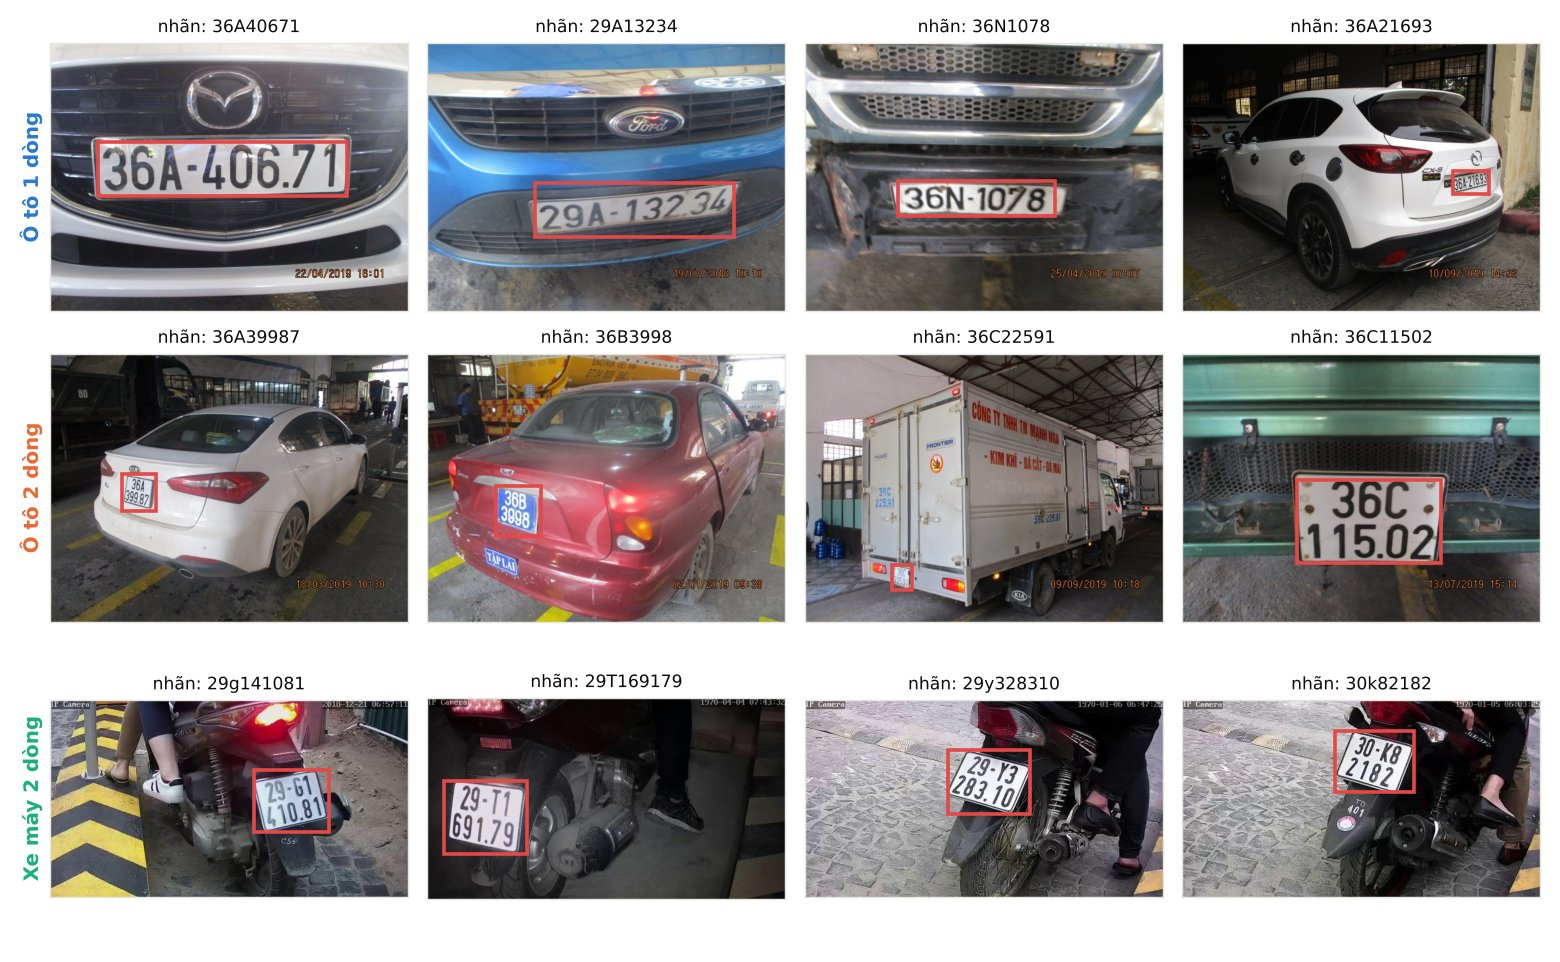
\includegraphics[width=\textwidth]{images/dataset/vnlp_samples.jpg}
\caption{Ảnh mẫu của ba nhóm dữ liệu VNLP (khung đỏ vẽ theo nhãn gốc)}
\label{fig:vnlp_samples}
\end{figure}

\subsection{Định dạng nhãn}

VNLP không có tệp nhãn riêng; toàn bộ thông tin nhãn được mã hóa trong tên tệp ảnh, các trường phân tách bằng dấu gạch dưới. Ví dụ với tệp \texttt{1\_1463\_1\_36C09130\_116\_312\_208\_368.jpg}:

\begin{itemize}
  \item Ba trường đầu (\texttt{1\_1463\_1}) là mã nội bộ, không dùng cho huấn luyện. Trường thứ ba nhận giá trị 1 với biển 1 dòng và 0 với biển 2 dòng.
  \item Trường thứ tư (\texttt{36C09130}) là chuỗi ký tự biển số, đã bỏ dấu gạch và dấu chấm.
  \item Bốn trường cuối (\texttt{116\_312\_208\_368}) là tọa độ hộp biển số.
\end{itemize}

Tài liệu đi kèm bộ dữ liệu ghi bốn số cuối là ``góc trên trái và chiều rộng, chiều cao''. Khi vẽ lại nhãn lên ảnh (Hình~\ref{fig:vnlp_samples}), nhóm xác nhận bốn số này thực chất là \textbf{tọa độ hai góc} $(x_{\min}, y_{\min}, x_{\max}, y_{\max})$: cách hiểu theo chiều rộng, chiều cao làm hộp vượt ra ngoài ảnh rộng 640 điểm ảnh. Đây là chi tiết bắt buộc phải xử lý đúng khi chuyển sang định dạng YOLO.

Trong mẫu 93 ảnh được kiểm tra, mọi ảnh có chiều rộng 640 điểm ảnh, chiều cao 480, 360 hoặc 352 điểm ảnh.

\subsection{Thống kê phân bố}

Hình~\ref{fig:vnlp_stats} tổng hợp các thống kê chính, tính trên toàn bộ 37.297 nhãn.

\begin{figure}[H]
\centering
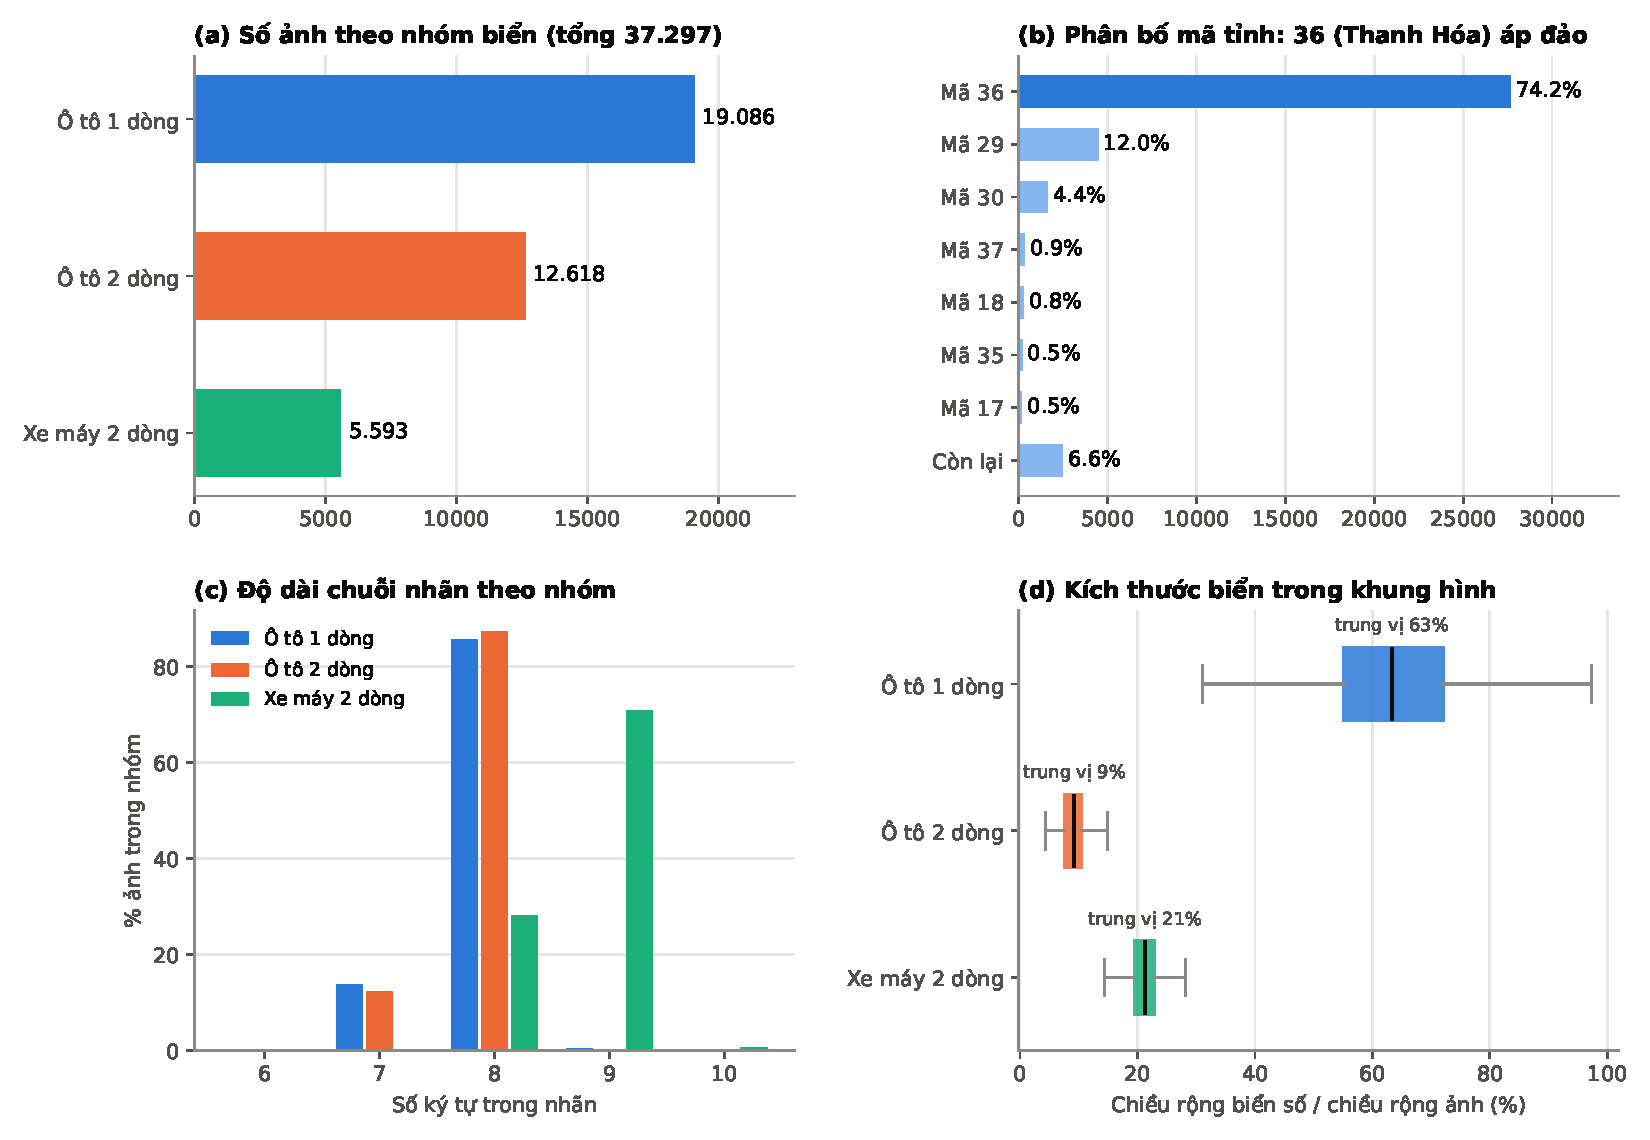
\includegraphics[width=\textwidth]{images/dataset/vnlp_stats.pdf}
\caption{Thống kê tập VNLP: (a) số ảnh theo nhóm, (b) mã tỉnh, (c) độ dài nhãn, (d) kích thước biển so với ảnh}
\label{fig:vnlp_stats}
\end{figure}

Từ Hình~\ref{fig:vnlp_stats} có thể rút ra:

\begin{itemize}
  \item \textbf{Mất cân bằng vùng miền:} biển mã 36 (Thanh Hóa) chiếm 74,2\% toàn bộ dữ liệu và khoảng 87\% ở hai nhóm ô tô; nhóm xe máy chủ yếu là mã 29 (Hà Nội). Các mã tỉnh khác rất ít mẫu.
  \item \textbf{Độ dài chuỗi khác nhau theo nhóm:} biển ô tô chủ yếu dài 8 ký tự (khoảng 86\%) hoặc 7 ký tự (biển cũ 4 số); biển xe máy chủ yếu dài 9 ký tự do seri gồm chữ và số (ví dụ \texttt{29G1-410.81}).
  \item \textbf{Kích thước biển chênh lệch rất lớn:} ở nhóm 1 dòng biển chiếm trung vị 63\% chiều rộng ảnh, trong khi ở nhóm 2 dòng ô tô chỉ chiếm khoảng 9\% (cao khoảng 64 điểm ảnh, có ảnh chỉ khoảng 30 điểm ảnh).
\end{itemize}

\subsection{Các vấn đề của tập dữ liệu}
\label{sec:vnlp_issues}

Khi rà soát nhãn và ảnh, nhóm phát hiện các vấn đề được minh họa trong Hình~\ref{fig:vnlp_issues} và tổng hợp trong Bảng~\ref{tab:vnlp_issues}.

\begin{figure}[H]
\centering
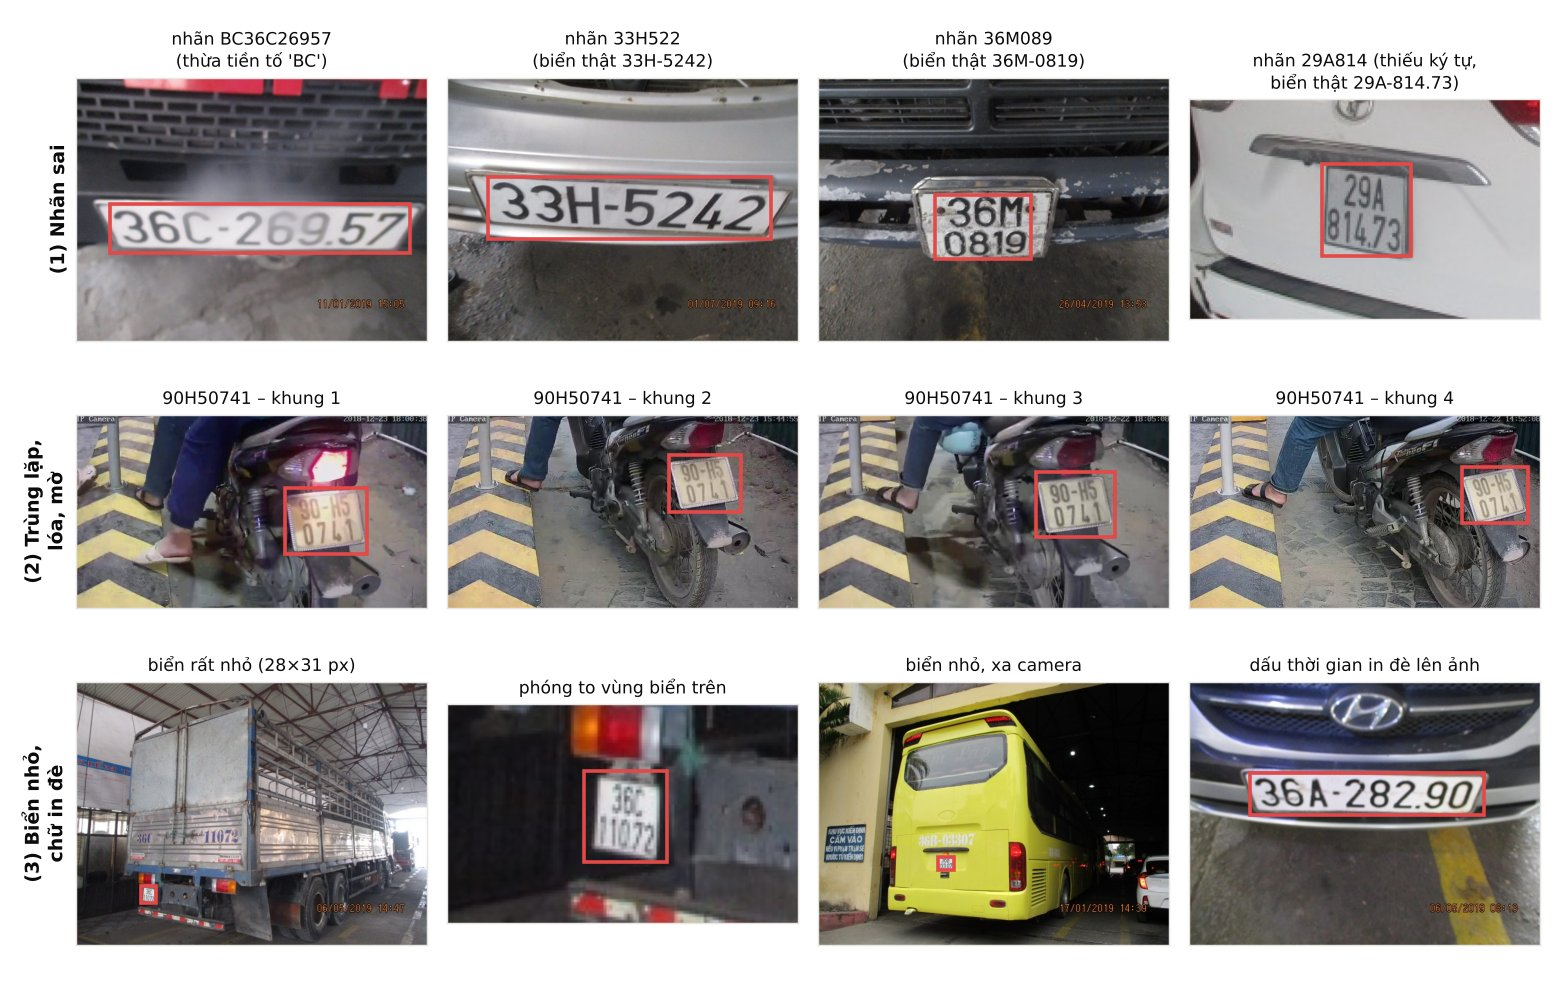
\includegraphics[width=\textwidth]{images/dataset/vnlp_issues.jpg}
\caption{Một số vấn đề của tập VNLP: nhãn sai, khung hình trùng lặp và lóa sáng, biển rất nhỏ, chữ in đè lên ảnh}
\label{fig:vnlp_issues}
\end{figure}

\begin{table}[H]
\centering
\small
\begin{tabularx}{\textwidth}{|>{\RaggedRight}p{3.3cm}|>{\RaggedRight}X|>{\RaggedRight\arraybackslash}p{5.0cm}|}
\hline
\textbf{Vấn đề} & \textbf{Biểu hiện, số liệu} & \textbf{Ảnh hưởng} \\
\hline
1. Lệch miền dữ liệu (domain gap) & Ảnh chụp trong nhà đăng kiểm, xe đứng yên, ánh sáng ổn định; không có cảnh đường phố, ban đêm, mưa; không có video ô tô & Mô hình đạt điểm cao trên VNLP nhưng có thể giảm mạnh khi chạy trên camera giao thông thật \\
\hline
2. Mất cân bằng mã tỉnh & 74,2\% biển mã 36 & Mô hình OCR thiên vị ký tự ``3'', ``6'' ở hai vị trí đầu, đọc kém biển tỉnh khác \\
\hline
3. Trùng lặp biển số & 29.304 ảnh (78,6\%) có biển số trùng với ít nhất một ảnh khác: cùng một ô tô chụp cả đầu và đuôi xe ở hai thư mục (10.465 biển); xe máy có biển xuất hiện tới 9 lần (khung hình liên tiếp) & Nếu chia ngẫu nhiên từng ảnh theo tỷ lệ 80/10/10, khoảng 66\% ảnh kiểm thử có cùng biển số trong tập huấn luyện; kết quả bị thổi phồng \\
\hline
4. Nhãn sai & 59 nhãn không khớp định dạng biển Việt Nam; đối chiếu từng ảnh: 37 nhãn sai (thừa chữ số như \texttt{36A041270}, thừa tiền tố như \texttt{BC36C26957}, thiếu ký tự như \texttt{29A814}, \texttt{33H522}), 21 nhãn đúng nhưng là định dạng đặc biệt, 1 nhãn không đọc được & Gây nhiễu khi huấn luyện OCR, làm sai lệch độ đo \\
\hline
5. Nhãn không đồng nhất & 3.715 nhãn dùng chữ thường (\texttt{29g141081}), chủ yếu ở nhóm xe máy & Nếu không chuẩn hóa, mô hình phải học hai lớp cho cùng một chữ cái \\
\hline
6. Tài liệu ghi sai định dạng tọa độ & Ghi $(x, y, w, h)$ nhưng thực tế là $(x_{\min}, y_{\min}, x_{\max}, y_{\max})$ & Chuyển đổi sai sẽ làm hỏng toàn bộ nhãn detection \\
\hline
7. Biển rất nhỏ, ảnh nhiễu & Biển 2 dòng ô tô chỉ chiếm khoảng 9\% chiều rộng ảnh; ảnh xe máy bị lóa đèn hậu, mờ; dấu thời gian in đè trên ảnh & Thách thức cho detector và OCR, nhưng cũng là dữ liệu khó có ích cho huấn luyện \\
\hline
\end{tabularx}
\caption{Tổng hợp các vấn đề của tập dữ liệu VNLP}
\label{tab:vnlp_issues}
\end{table}

\subsection{Hướng xử lý dữ liệu}

Từ các vấn đề trên, nhóm đề ra quy trình xử lý dữ liệu như Bảng~\ref{tab:vnlp_solutions}.

\begin{table}[H]
\centering
\small
\begin{tabularx}{\textwidth}{|>{\centering}p{0.8cm}|>{\RaggedRight\arraybackslash}X|}
\hline
\textbf{Vấn đề} & \textbf{Hướng xử lý} \\
\hline
1 & Xây dựng thêm 300--1.000 khung hình từ nguồn bên ngoài VNLP: video giao thông Việt Nam công khai có giấy phép phù hợp (ví dụ Creative Commons) và các bộ dữ liệu công khai khác (Roboflow Universe, GreenParking), ưu tiên cảnh đường phố, ban đêm, trời mưa; gán nhãn bằng Roboflow hoặc CVAT và loại các ảnh trùng với VNLP. Bộ này dùng làm \textbf{tập kiểm thử thực tế} độc lập; một phần nhỏ có thể dùng tinh chỉnh detector. Kết quả được báo cáo riêng trên tập VNLP và trên tập thực tế. \\
\hline
2 & Báo cáo độ chính xác riêng cho nhóm biển mã 36 và nhóm mã tỉnh khác. Khi huấn luyện OCR, cân nhắc lấy mẫu lại (oversampling) các biển ngoài mã 36 và tạo thêm ảnh biển tổng hợp với mã tỉnh ngẫu nhiên. \\
\hline
3 & \textbf{Chia train/val/test theo chuỗi biển số} (group split): mọi ảnh của cùng một biển (kể cả ảnh đầu xe và đuôi xe của cùng một ô tô) chỉ nằm trong một tập. Tỷ lệ 80/10/10, phân tầng theo ba nhóm dữ liệu. \\
\hline
4 & Kiểm tra mọi nhãn bằng biểu thức chính quy theo định dạng biển (ô tô, xe máy, xe máy điện, xe máy kiểu cũ, biển nước ngoài); đối chiếu từng nhãn không khớp với ảnh. Đã sửa 37 nhãn sai (Hình~\ref{fig:vnlp_label_fixes}); nhãn không đọc được bị loại khỏi tập OCR nhưng vẫn giữ cho detection. Kiểm tra thêm 89 ảnh mẫu có nhãn đúng định dạng: không phát hiện nhãn sai. \\
\hline
5 & Chuẩn hóa toàn bộ nhãn về chữ in hoa, bộ ký tự gồm 10 chữ số và các chữ cái dùng trên biển Việt Nam. \\
\hline
6 & Viết script chuyển đổi đọc tọa độ theo định dạng hai góc, vẽ ngẫu nhiên 50 ảnh để kiểm tra trực quan trước khi huấn luyện. \\
\hline
7 & Giữ lại ảnh khó; huấn luyện detector ở kích thước 640 để không mất biển nhỏ. Tăng cường dữ liệu trực tuyến trong lúc huấn luyện (mờ chuyển động, đổi sáng, nhiễu, xoay nhẹ) thay vì tạo sẵn ảnh tăng cường. \\
\hline
\end{tabularx}
\caption{Hướng xử lý tương ứng với từng vấn đề dữ liệu}
\label{tab:vnlp_solutions}
\end{table}

\begin{figure}[H]
\centering
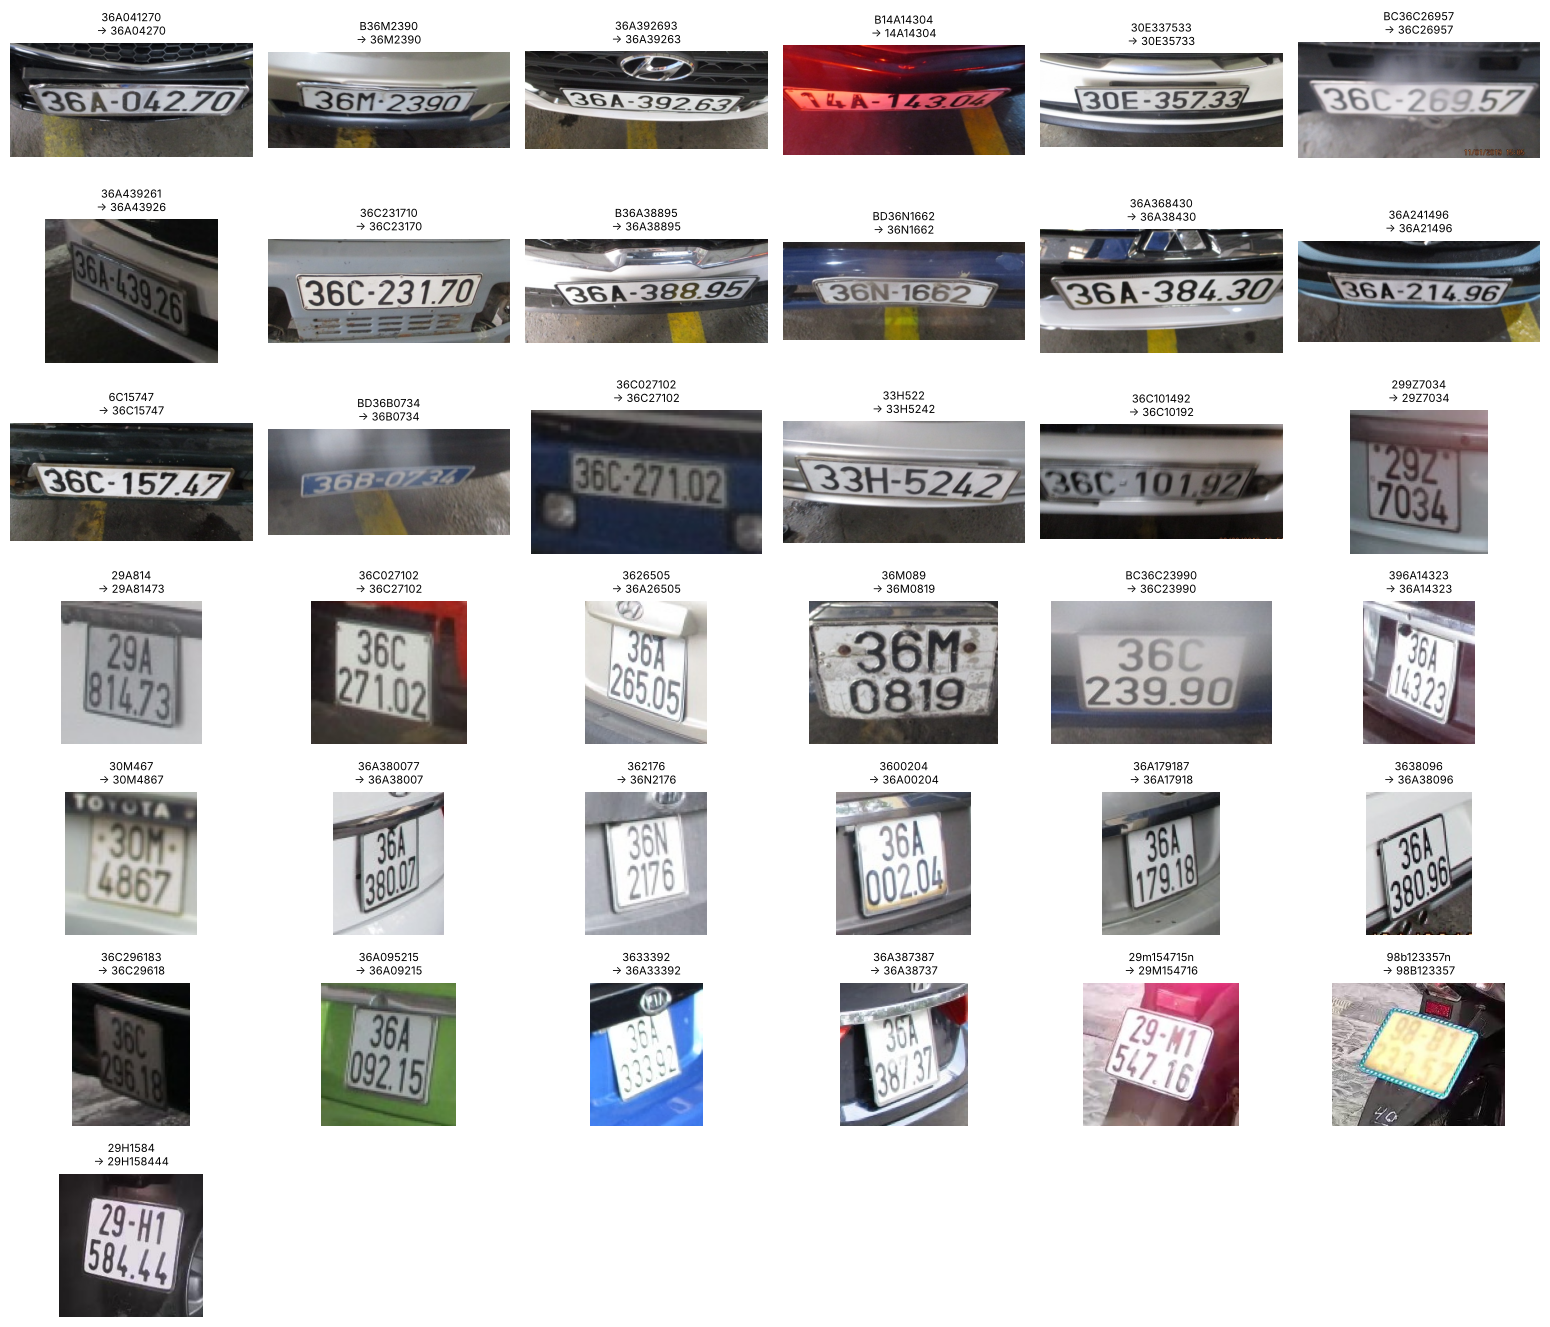
\includegraphics[width=0.95\textwidth]{images/dataset/vnlp_label_fixes.png}
\caption{37 nhãn sai đã được sửa: dòng trên là nhãn gốc, dòng dưới là nhãn sau khi đối chiếu với ảnh}
\label{fig:vnlp_label_fixes}
\end{figure}

Sau xử lý, từ VNLP sinh ra hai bộ dữ liệu dùng chung một cách chia:
\begin{enumerate}
  \item \textbf{Bộ detection:} ảnh gốc kèm tệp nhãn YOLO \texttt{(class, x\_center, y\_center, w, h)} chuẩn hóa về $[0, 1]$, gồm 2 lớp: \texttt{plate\_1row} và \texttt{plate\_2row}.
  \item \textbf{Bộ nhận dạng ký tự:} ảnh biển số được cắt theo hộp nhãn (thêm lề 3--5\%) kèm chuỗi ký tự đã chuẩn hóa.
\end{enumerate}

\section{Xác định đầu vào, đầu ra và yêu cầu của hệ thống}

\subsection{Đầu vào}

Hệ thống hỗ trợ ba loại đầu vào: ảnh tĩnh tải lên từ máy tính, tệp video và luồng webcam trực tiếp. Hệ thống cần hỗ trợ định dạng phổ biến (JPG, PNG, MP4) và thông báo rõ ràng khi tệp không hợp lệ hoặc không thể xử lý.

\subsection{Đầu ra}

Đầu ra dự kiến gồm:

\begin{itemize}
  \item Ảnh hoặc khung hình có vùng biển số được khoanh, kèm chuỗi ký tự hiển thị phía trên.
  \item Chuỗi biển số đã chuẩn hóa theo định dạng Việt Nam (ví dụ ``30A-123.45'').
  \item Điểm tin cậy của bước phát hiện và độ tin cậy của chuỗi ký tự.
  \item Với video: danh sách phương tiện kèm mã theo dõi, thời điểm xuất hiện và biển số cuối cùng sau tổng hợp.
  \item Thông báo phù hợp nếu không phát hiện được biển số hoặc không đọc được ký tự.
\end{itemize}

Cần phân biệt điểm tin cậy của mô hình phát hiện với xác suất chuỗi biển số được nhận dạng chính xác. Hai đại lượng này không đồng nghĩa với nhau.

\subsection{Yêu cầu chức năng}

Hệ thống cần đáp ứng các yêu cầu chức năng cơ bản:

\begin{enumerate}
  \item Cho phép tải ảnh, tải video hoặc mở webcam.
  \item Kiểm tra tính hợp lệ của tệp đầu vào.
  \item Phát hiện vị trí và loại biển số.
  \item Nhận dạng ký tự trên biển và chuẩn hóa theo định dạng biển Việt Nam.
  \item Theo dõi phương tiện và tổng hợp kết quả qua nhiều khung hình với đầu vào video.
  \item Hiển thị kết quả và lưu lịch sử nhận dạng.
  \item Cung cấp liên kết đến trang tra cứu vi phạm chính thức kèm biển số đã nhận dạng để người dùng tự tra cứu.
\end{enumerate}

\subsection{Yêu cầu phi chức năng}

\begin{itemize}
  \item \textbf{Độ chính xác:} hạn chế phát hiện nhầm và đọc sai ký tự; được đo trên cả tập VNLP và tập thực tế.
  \item \textbf{Thời gian thực:} xử lý webcam ở tốc độ từ 15 khung hình/giây trở lên trên máy tính xách tay của nhóm (mục tiêu sẽ được xác nhận bằng thực nghiệm).
  \item \textbf{Khả năng sử dụng:} giao diện web đơn giản, chạy được trên trình duyệt.
  \item \textbf{Chi phí triển khai:} sử dụng hạ tầng miễn phí, phù hợp với điều kiện sinh viên.
  \item \textbf{Bảo vệ dữ liệu:} biển số là dữ liệu liên quan đến cá nhân; hệ thống không chia sẻ ảnh, không tự động truy vấn hệ thống bên thứ ba.
\end{itemize}

\section{Lựa chọn công nghệ và giải pháp}

\subsection{Ngôn ngữ lập trình Python}

Python được lựa chọn làm ngôn ngữ chính do có hệ sinh thái phong phú cho thị giác máy tính và học sâu (PyTorch, OpenCV, Ultralytics), cho phép thực hiện toàn bộ quy trình từ xử lý dữ liệu, huấn luyện đến xây dựng dịch vụ trong một ngôn ngữ.

\subsection{OpenCV -- Xử lý ảnh}

OpenCV đảm nhiệm đọc ảnh và video, thay đổi kích thước, cắt vùng biển số và vẽ kết quả. OpenCV không tự giải quyết bài toán nhận dạng mà được kết hợp với các mô hình học sâu.

\subsection{YOLO và RT-DETR -- Phát hiện biển số}

Thư viện Ultralytics cung cấp cùng một giao diện huấn luyện cho các họ mô hình YOLO (YOLO11, YOLO26) và RT-DETR. Do mô hình huấn luyện sẵn trên tập COCO không có lớp biển số, nhóm tinh chỉnh các mô hình này trên tập VNLP đã chuyển đổi.

\subsection{Mô hình nhận dạng ký tự}

Các công cụ OCR tổng quát như Tesseract hay EasyOCR được thiết kế cho văn bản thông thường, thường đọc kém biển số 2 dòng. Nhóm dùng chúng làm mốc so sánh (baseline) và lựa chọn hướng chính là \textbf{huấn luyện mô hình nhận dạng cả biển} trên ảnh biển cắt từ VNLP (CRNN với hàm mất mát CTC, hoặc tinh chỉnh mô hình nhẹ chuyên cho biển số như \texttt{fast-plate-ocr}). Mô hình đọc cả biển trong một lần, không cần tách từng ký tự hay tách dòng.

\subsection{Giao diện và triển khai}

Giao diện được xây dựng dưới dạng ứng dụng web gồm máy chủ FastAPI xử lý ảnh, video và giao diện trình duyệt hiển thị kết quả. Mô hình được xuất sang định dạng ONNX để suy luận nhanh trên CPU hoặc GPU của máy cá nhân. Streamlit có thể dùng cho bản trình diễn nhanh trong giai đoạn đầu.

\subsection{Giải pháp tổng thể}

Giải pháp được lựa chọn là quy trình nhiều bước:

\begin{enumerate}
  \item \textbf{Tiếp nhận đầu vào:} ảnh, video hoặc khung hình webcam.
  \item \textbf{Phát hiện biển số:} mô hình phát hiện trả về hộp biển và loại biển.
  \item \textbf{Cắt và chuẩn hóa:} cắt vùng biển có thêm lề, đổi kích thước theo loại biển.
  \item \textbf{Nhận dạng ký tự:} mô hình nhận dạng trả về chuỗi và độ tin cậy.
  \item \textbf{Hậu xử lý:} kiểm tra và sửa theo định dạng biển Việt Nam.
  \item \textbf{Theo dõi và tổng hợp (với video):} gán mã cho từng xe, bỏ phiếu kết quả qua nhiều khung hình.
  \item \textbf{Hiển thị và lưu kết quả.}
\end{enumerate}

Thiết kế này tách rõ các thành phần, giúp kiểm thử từng bước và xác định nguyên nhân khi kết quả cuối cùng sai: do phát hiện, do vùng cắt hay do nhận dạng ký tự.

\section{Tiêu chí đánh giá hiệu quả giải pháp}

Hệ thống được đánh giá cả về khả năng phát hiện biển số và khả năng đọc đúng nội dung biển số.

Precision đo tỷ lệ dự đoán đúng trong tổng số dự đoán:
\[
  \mathrm{Precision} = \frac{TP}{TP + FP}
\]
Recall đo tỷ lệ biển số thực tế được phát hiện:
\[
  \mathrm{Recall} = \frac{TP}{TP + FN}
\]
trong đó TP là số biển phát hiện đúng, FP là số phát hiện nhầm và FN là số biển bị bỏ sót.

mAP@0.5 và mAP@0.5:0.95 đánh giá chất lượng hộp giới hạn; mAP@0.5:0.95 đặc biệt quan trọng vì hộp lệch có thể cắt mất ký tự sát mép.

Tỷ lệ đọc đúng toàn biển (Exact Match Accuracy) đo tỷ lệ mẫu có chuỗi dự đoán trùng hoàn toàn với nhãn:
\[
  \mathrm{Exact\ Match\ Accuracy} = \frac{\text{Số chuỗi đúng hoàn toàn}}{\text{Tổng số mẫu kiểm thử}}
\]

Ngoài ra, nhóm đo tỷ lệ lỗi ký tự (CER) và tốc độ xử lý (khung hình/giây). Mọi chỉ số được tính trên tập kiểm thử độc lập và \textbf{báo cáo riêng cho tập VNLP và tập thực tế}. Báo cáo chỉ trình bày kết quả thực nghiệm thực tế, không tự đặt ra giá trị khi chưa đánh giá.
   % 2. Phân tích bài toán thực tế
\chapter{THIẾT KẾ GIẢI PHÁP VÀ MÔ HÌNH HỌC MÁY, MÔ HÌNH AI, GIẢI THUẬT}

\section{Xây dựng thuật toán/mô hình}

\section{Quy trình xử lý dữ liệu}

   % 3. Thiết kế giải pháp và mô hình
\chapter{TRIỂN KHAI VÀ KẾT QUẢ THỰC HIỆN}

\section{Kế hoạch triển khai và dự kiến kết quả thực hiện}

Do dự án đang trong giai đoạn thiết kế giải pháp, quy trình triển khai thực nghiệm được nhóm định hướng theo các bước như sau:

\subsection{Kế hoạch cài đặt thực nghiệm}
\begin{itemize}
  \item \textbf{Môi trường và công cụ phát triển:}
  \begin{itemize}
    \item Ngôn ngữ lập trình: Python (hỗ trợ mạnh mẽ các thư viện học máy và học sâu).
    \item Môi trường huấn luyện: Sử dụng Google Colab hoặc máy tính cá nhân có hỗ trợ GPU để tăng tốc quá trình huấn luyện mạng nơ-ron (CNN).
    \item Thư viện/Framework dự kiến: OpenCV (để tiền xử lý ảnh), PyTorch hoặc TensorFlow (để xây dựng kiến trúc mô hình học sâu).
  \end{itemize}

  \item \textbf{Kế hoạch triển khai mã nguồn:}
  \begin{itemize}
    \item Bước 1 (Phát hiện biển số - Detection): Triển khai mã nguồn họ mô hình YOLO (dự kiến YOLOv8) để nhận diện vùng chứa biển số trong khung hình và cắt (crop) vùng đó ra.
    \item Bước 2 (Tiền xử lý ảnh): Viết các hàm (functions) xử lý ảnh crop như chuyển đổi sang thang độ xám (grayscale), nhị phân hóa và căn chỉnh góc nghiêng.
    \item Bước 3 (Nhận diện ký tự - Recognition): Cài đặt mô hình CRNN (Convolutional Recurrent Neural Network) hoặc sử dụng các thư viện OCR tinh chỉnh cho font chữ biển số Việt Nam để xuất ra chuỗi ký tự text cuối cùng.
  \end{itemize}
\end{itemize}

\subsection{Kịch bản thử nghiệm và các độ đo đánh giá (Dự kiến)}
\begin{itemize}
  \item \textbf{Kịch bản chạy thử nghiệm:}
  \begin{itemize}
    \item Kịch bản lý tưởng: Mô hình nhận diện chính xác các ảnh biển số (ô tô/xe máy) chụp thẳng, rõ nét, đầy đủ ánh sáng ban ngày.
    \item Kịch bản thách thức: Đưa vào hệ thống các dữ liệu thực tế khó như: ảnh chụp vào ban đêm (bị lóa đèn), ảnh chụp góc nghiêng, góc khuất, biển số bị bám bùn đất hoặc bị lóa sáng do thời tiết.
  \end{itemize}

  \item \textbf{Đánh giá mô hình (Thông số định lượng):}
  \begin{itemize}
    \item Đánh giá bài toán Phát hiện (Detection): Sử dụng độ đo định lượng mAP (Mean Average Precision) và IoU (Intersection over Union) để đo độ chính xác của khung bao (bounding box) bắt được biển số.
    \item Đánh giá bài toán Nhận diện (Recognition): Sử dụng Accuracy (Độ chính xác tổng thể), CER (Character Error Rate - Tỷ lệ lỗi ký tự) và giám sát hàm mất mát (Loss) trong quá trình huấn luyện để đánh giá sự hội tụ của mô hình.
  \end{itemize}
\end{itemize}

\subsection{Phân tích và nhận xét (Hướng so sánh dự kiến)}
\begin{itemize}
  \item \textbf{So sánh giữa các phương pháp:} Dựa trên tập dữ liệu chuẩn bị, nhóm dự kiến sẽ huấn luyện song song hai hoặc nhiều cấu trúc mô hình mạng CNN khác nhau (ví dụ: so sánh tốc độ, độ hiệu quả giữa YOLOv8 và Faster R-CNN cho tác vụ bắt biển số) để đưa ra đánh giá khách quan.

  \item \textbf{Tiêu chí phân tích:} Việc phân tích sẽ tập trung vào sự đánh đổi (trade-off) giữa độ chính xác nhận diện và thời gian xử lý (tốc độ FPS). Từ đó, nhóm sẽ đưa ra nhận xét và lựa chọn mô hình tối ưu nhất để có thể ứng dụng vào các hệ thống thời gian thực (như barrier thông minh, camera bãi giữ xe).
\end{itemize}

   % 4. Triển khai và kết quả thực hiện
\chapter{KẾT LUẬN VÀ HƯỚNG PHÁT TRIỂN}

\section{Đánh giá ưu điểm và nhược điểm}

\section{Hướng phát triển}

   % 5. Kết luận và hướng phát triển
\chapter*{TÀI LIỆU THAM KHẢO}
\addcontentsline{toc}{chapter}{Tài liệu tham khảo}



\end{document}
